% Created 2021-02-26 vie 16:10
% Intended LaTeX compiler: pdflatex
\documentclass[presentation,aspectratio=169]{beamer}
\usepackage[utf8]{inputenc}
\usepackage[T1]{fontenc}
\usepackage{graphicx}
\usepackage{grffile}
\usepackage{longtable}
\usepackage{wrapfig}
\usepackage{rotating}
\usepackage[normalem]{ulem}
\usepackage{amsmath}
\usepackage{textcomp}
\usepackage{amssymb}
\usepackage{capt-of}
\usepackage{hyperref}
\usepackage{khpreamble}
\usepackage{amssymb}
\usepgfplotslibrary{groupplots}
\newcommand*{\shift}{\operatorname{q}}
\DeclareMathSymbol{\Omega}{\mathalpha}{letters}{"0A}% italics
\DeclareMathSymbol{\varOmega}{\mathalpha}{operators}{"0A}% upright
\providecommand*{\upOmega}{\varOmega}% for siunitx
\usepackage[binary-units=true]{siunitx}
\usepackage{circuitikz}
\usetheme{default}
\author{Kjartan Halvorsen}
\date{2021-03-01}
\title{Actuadores}
\hypersetup{
 pdfauthor={Kjartan Halvorsen},
 pdftitle={Actuadores},
 pdfkeywords={},
 pdfsubject={},
 pdfcreator={Emacs 26.3 (Org mode 9.4.4)}, 
 pdflang={English}}
\begin{document}

\maketitle

\section{Requerimientos mecanicos}
\label{sec:org54ca95e}

\begin{frame}[label={sec:orgbe1f6cb}]{Requerimientos mecanicos}
\end{frame}
\begin{frame}[label={sec:org8412c57}]{Energía mecanica}
From Encyclopaedia Britannica
\begin{quote}
\alert{Mechanical energy}, sum of the kinetic energy, or energy of motion, and the potential energy, or energy stored in a system by reason of the position of its parts. 
\end{quote}

\[ E_M = \underbrace{K}_{\text{Kinetic energy}} + \underbrace{U}_{\text{Potential energy}}\]

For a point mass \(m\) with velocity \(v\) at a height \(h\) above reference level, the mechanical energy is \(E_M = \frac{1}{2}mv^2 + mgh\).

\begin{center}
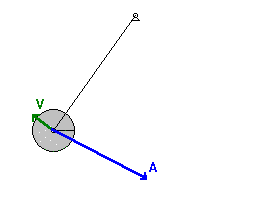
\includegraphics[height=0.3\textheight]{../../figures/pendulum.png}
{\footnotesize CC-BY-SA Hubert Christiaen, wikipedia}
\end{center}


\#+end\textsubscript{center}
\end{frame}
\begin{frame}[label={sec:orgd3b5f93}]{Trabajo}
From Encyclopaedia Britannica
\begin{quote}
\alert{Work}, in physics, measure of \alert{energy transfer} that occurs when an object is \alert{moved over a distance} by an \alert{external force} at least part of which is applied in the direction of the displacement.
\end{quote}
\end{frame}

\begin{frame}[label={sec:org5d0666f}]{Trabajo}
\begin{center}
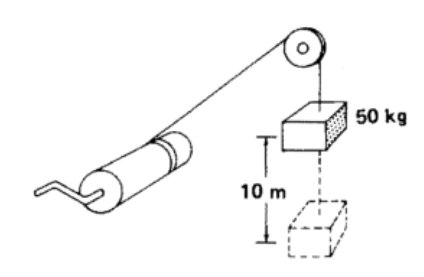
\includegraphics[height=0.6\textheight]{../../figures/pulley-block-50kg.png}
\end{center}

\alert{Actividad individual 1} Se levanta un cuerpo de \unit{50}{\kilogram} una distancia de \unit{10}{\meter}. Calcula el trabajo realizado. Manda tu respuesta en el chat.
\end{frame}



\begin{frame}[label={sec:org6c03b17}]{Potencia}
\alert{Definition} The rate of work done, or the time-derivative of the work.
\end{frame}

\begin{frame}[label={sec:org8aad4e3}]{Potencia}
\begin{center}
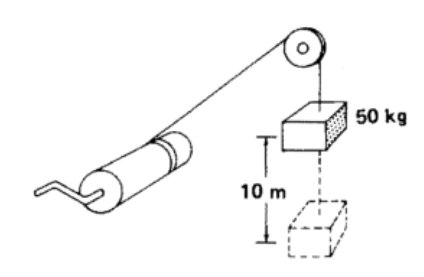
\includegraphics[height=0.6\textheight]{../../figures/pulley-block-50kg.png}
\end{center}

\alert{Individual exercise 2} A mass of \unit{50}{\kilogram} is lifted \unit{10}{\meter} with constant velocity \unit{2}{\meter\per\second}. Calculate the power required if all frictional forces can be ignored. Answer in chat directly to host.
\end{frame}

\begin{frame}[label={sec:orgb583224}]{Potencia y fuerza para accelerar}
   \begin{center}
\begin{tikzpicture}

  \begin{scope}[scale=0.3, xshift=4cm]
  \node[anchor=south,] {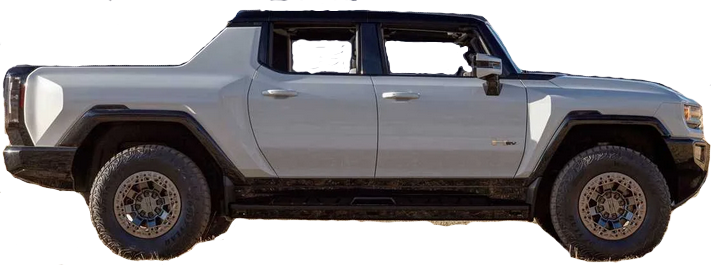
\includegraphics[width=3cm]{../../figures/hummer-ev.png}};
    \draw[thin, ] (-8,2) -- (-6,2);
    \draw[thin, ] (-9,3) -- (-6.5,3);
  \end{scope}

  \draw[->,semithick] (-.5,0.16) -- (8,0.16);
\end{tikzpicture}
\end{center}


\alert{Individual exercise} El nuevo Hummer EV tiene una masa de \(m=\unit{5000}{\kilogram}\), y puede accelerarar de \unit{0 - 100}{\kilo\meter\per\hour} en tres segundos. Cual es la potencia mediana necesario para rograr esto (ignorando la resistencia del aire y ra resistencia a la rodura)?
\end{frame}

\begin{frame}[label={sec:org919d2eb}]{Potencia en rotación}
\alert{Torque} times \alert{angular velocity}

\begin{center}
  \begin{tikzpicture}

  \begin{scope}[scale=1, xshift=2cm, yshift=2cm]
    \node[] {\includegraphics[width=2cm]{../../figures/mech-rotor}};
    \node[green!80!black] at (2.6,0) {Driving forward};
    \end{scope}

  \begin{scope}[scale=1, xshift=-2cm, yshift=2cm]
    \node[] {\includegraphics[width=2cm]{../../figures/mech-motor-back-break}};
    \node[red!80!black, anchor=east] at (-2,0) {Braking};
  \end{scope}

  \begin{scope}[scale=1, xshift=-2cm, yshift=-2cm]
    \node[] {\includegraphics[width=2cm]{../../figures/mech-motor-back}};
    \node[green!80!black, anchor=east] at (-2,0) {Driving backward};
  \end{scope}

  \begin{scope}[scale=1, xshift=2cm, yshift=-2cm]
    \node[] {\includegraphics[width=2cm]{../../figures/mech-rotor-break}};
    \node[red!80!black] at (2.6,0) {Braking};
  \end{scope}

  \draw[->,semithick] (-3, 0) -- (3, 0) node[right] {$\omega$};
  \draw[->,semithick] (0, -3) -- (0, 3) node[above] {$T$};
\end{tikzpicture}
\end{center}
\end{frame}



\begin{frame}[label={sec:org61217a8}]{Inercia}
The tendency of a body to resist angular acceleration.
\[ J \dot{\omega} = \sum T_i \]

\begin{center}
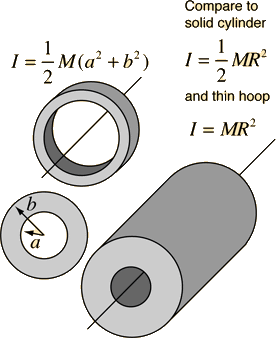
\includegraphics[height=0.6\textheight]{../../figures/moment-of-inertia-cylinder.png}
{\footnotesize Georgia State University, CC-By-SA}
\end{center}
\end{frame}

\begin{frame}[label={sec:org059f373}]{Inercia - usando la energía cinética}
For point masses we have kinetic energy \[K = \frac{1}{2}\textcolor{red!80!black}{m}v^2\]
 and for rotating bodies we have kinetic energy
\[ K = \frac{1}{2}\textcolor{red!80!black}{J}\omega^2.\]

In both cases we can identify the inertia (mass or moment of inertia) directly from the expression
for the kinetic energy.
\end{frame}


\begin{frame}[label={sec:orgfd486f6}]{Inercia}
\begin{center}
\includegraphics[width=0.6\textwidth]{../../figures/mech-mass-on-band}
\end{center}

Assume pulleys have moment of inertia \(J_p\), mass \(m\) includes the mass of the band and the box, the rotor  has moment of inertia \(J_m\). The belt velocity and the angular velocities are related as \(\omega_mr = \omega_pR = v\).  

The total kinetic energy is the sum of the kinetic energy in the different moving bodies
\begin{align*}
K &= \frac{1}{2}(2J_p)\omega_p^2 + \frac{1}{2}J_m\omega_m^2 + \frac{1}{2}m v^2
 = J_p\big(\frac{r}{R}\omega_m\big)^2 + \frac{1}{2}J_m\omega_m^2 + \frac{1}{2}m(r\omega_m)^2\\
 &= \frac{1}{2}(\underbrace{\textcolor{red!80!black}{J_m + 2(\frac{r}{R})^2J_p + mr^2}}_{\text{Inertia experienced by motor}}) \omega_m^2.
\end{align*}
\end{frame}

\begin{frame}[label={sec:org8a9e0af}]{Requerimientos de potencia y torque de un elevador}
\begin{columns}
\begin{column}{0.38\columnwidth}
\begin{center}
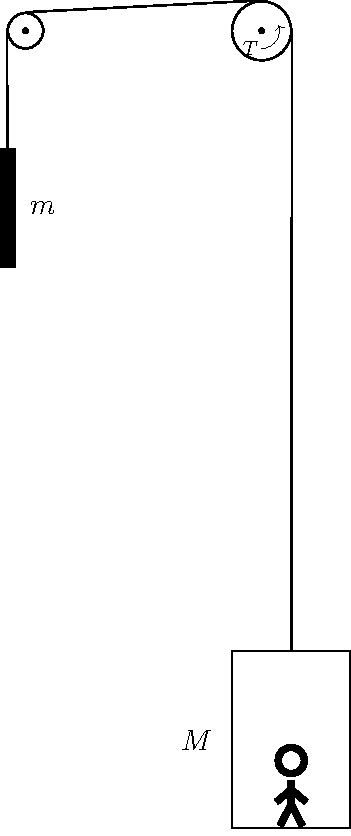
\includegraphics[height=0.8\textheight]{../../figures/mech-elevator}
\end{center}
\end{column}

\begin{column}{0.72\columnwidth}
\alert{Group exercise 1} Assume that the mass of the elevator with people is \(M=\unit{1000}{\kilogram}\) and that the counterweight has mass \(m=\unit{800}{\kilogram}\). The drive pulley has a radius of \(r=\unit{0.4}{\meter}\) and a moment of inertia of \(J_p = \unit{10}{\kilogram\meter\squared}\). The drive pulley is connected to an electric motor with a gear ratio of 1:12 (the motor rotates 12 times for every rotation of the pulley) The rotor of the motor has a moment of inertia of \(J_m = \unit{0.3}{\kilogram\meter\squared}\).

Determine: \alert{(a)} The inertia of the system as seen by the motor. \alert{(b)} The power required to move the elevator upwards at a constant speed of \unit{4}{\meter\per\second}. \alert{(c)} The average power required to accelerate the elevator from 0 to \unit{4}{\meter\per\second} in \unit{2}{\second} (hint: in this time the elevator has moved upwards \unit{4}{\meter}).
\end{column}
\end{columns}
\end{frame}


\section{El Motor electrico de corriente continua}
\label{sec:orgf547358}
\begin{frame}[label={sec:orgeb455fe}]{El Motor eléctrico de corriente continua}
\begin{center}
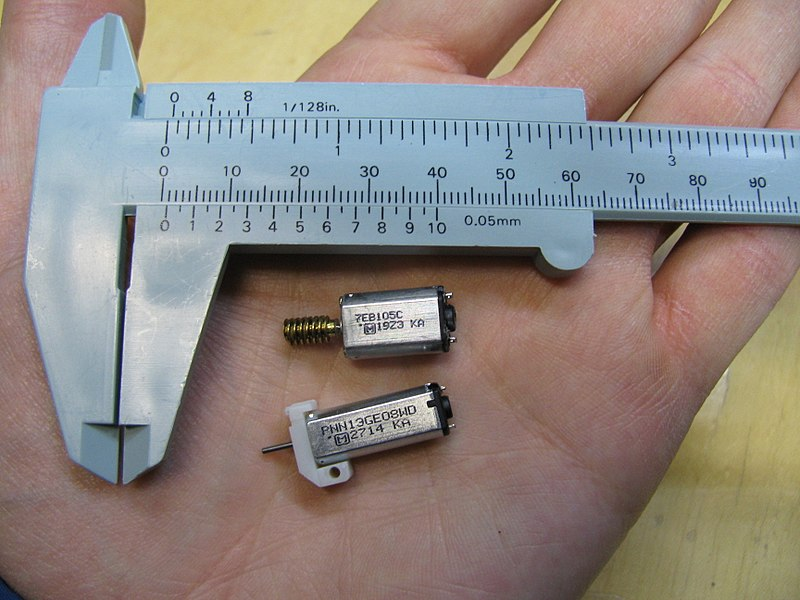
\includegraphics[height=0.6\textheight]{../../figures/wiki-small-dc-motor.jpg}
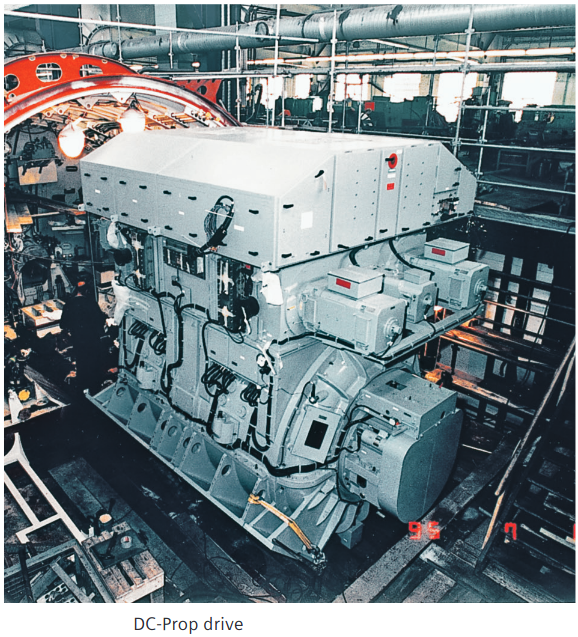
\includegraphics[width=0.6\textheight]{../../figures/Siemens-DC-prop.png}\\
{\footnotesize Fuente: Wikipedia \hspace*{3cm} Fuente: Siemens AG}
\end{center}
\end{frame}


\begin{frame}[label={sec:orga50de8e}]{Fuerza en un conductor eléctrico en un campo magnético}
\begin{center}
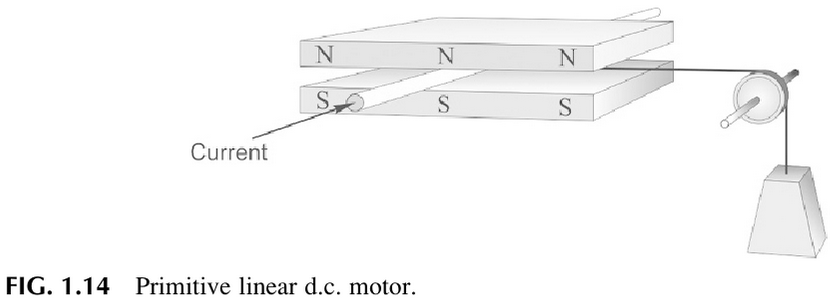
\includegraphics[width=0.4\linewidth]{../../figures/HD-fig1_14.png}
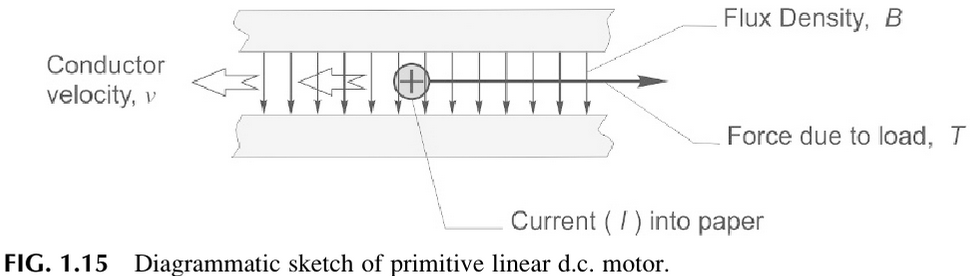
\includegraphics[width=0.53\linewidth]{../../figures/HD-fig1_15.png}
\end{center}


\begin{block}{Fuente}
\begin{center}
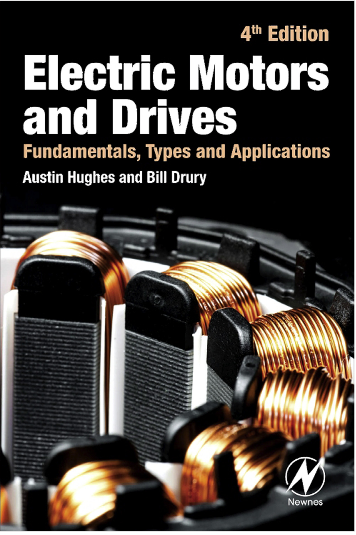
\includegraphics[width=0.2\linewidth]{../../figures/textbook.png}
\end{center}
\end{block}
\end{frame}


\begin{frame}[label={sec:orgda42239}]{Fuerza en un conductor eléctrico en un campo magnético}
\begin{center}
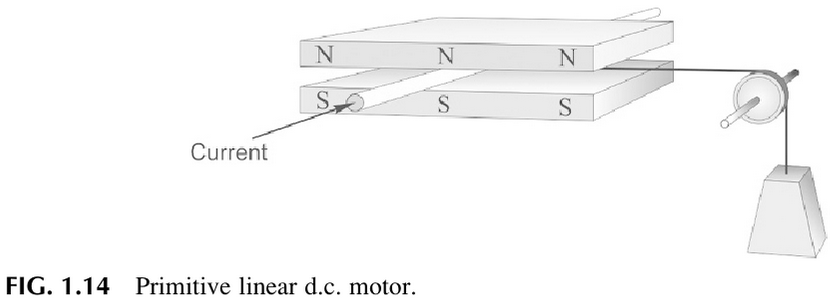
\includegraphics[width=0.4\linewidth]{../../figures/HD-fig1_14.png}
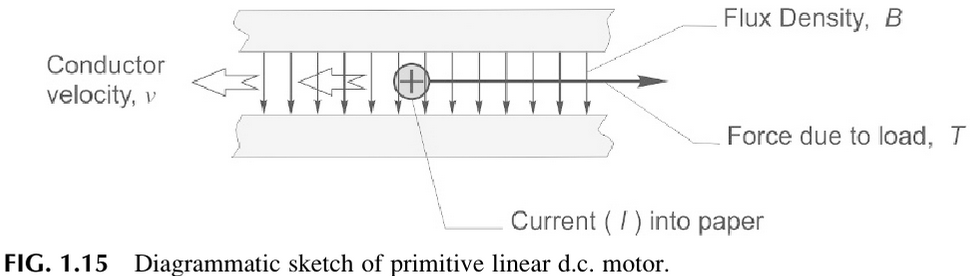
\includegraphics[width=0.53\linewidth]{../../figures/HD-fig1_15.png}
\end{center}

La fuerza electromagnetética en el conductor es proportional a la corriente: \(F=k_mI=(Bl_m)I\), donde \(B\) es la densidad del flujo magnético en el entrehierro, \(I\) es la corriente, y \(l_m\) es la longitud del cable. En vez de construir un motor muy larga, se agreaga varias cables juntos para aumentar la fuerza.

\alert{Actividad individual} En un motor grande de \unit{4}{\mega\watt} con longitud axial de \(l_m=\unit{2}{\meter}\), la densidad del flujo es \(B=\unit{0.8}{\tesla}\) y la corriente nominal en uso continuo es \(I=\unit{3}{\kilo\ampere}\). ¿Cuantas cables en paralelo se necesita para alcanzar una fuerza de \(F=\unit{259.2}{\kilo\newton}\)?
\end{frame}

\begin{frame}[label={sec:org8b8ec57}]{Las dos ecuaciónes del motor eléctrica CC}
\begin{block}{Fuerza generado por la corriente en el campo magnético}
\[ F(t) = k_m i(t) \quad\Leftrightarrow\quad T(t) = k_m r i(t),\]
dónde \(r\) es el radie del motor.
\end{block}

\begin{block}{Voltaje generado por el movimiento del conductor en el campo magnético}
\[ e(t) = k_v v(t) \quad\Leftrightarrow\quad e(t) = k_v r \omega(t)\]
\(e(t)\) se llama \emph{Fuerza contraelectromotriz} o \emph{Back electro-motive force (Back e.m.f.)} en inglés.
\end{block}
\end{frame}
\begin{frame}[label={sec:org5199a93}]{Potencia eléctrica y mecánica}
\begin{center}
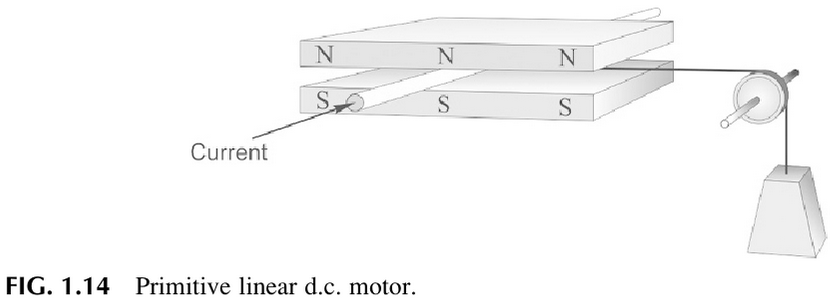
\includegraphics[width=0.4\linewidth]{../../figures/HD-fig1_14.png}
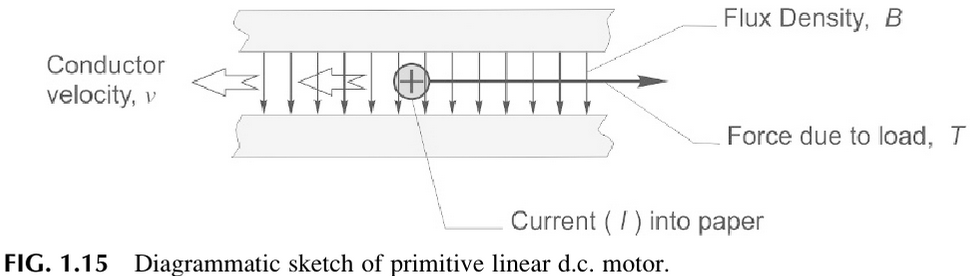
\includegraphics[width=0.53\linewidth]{../../figures/HD-fig1_15.png}
\end{center}

Con velocidad \(v\) constante y ignorando fricción y resistencia eléctrica: 

\[ \text{Fuerza electromagnética} = \text{Fuerza mecánica} \quad\Leftrightarrow\quad F=k_mI =Bl_mI = mg\]
\[ \text{Potencia electromag} = \text{Potencia mecánica} \quad \Leftrightarrow\quad \underbrace{V_1I}_{P_e} = \underbrace{Fv = Bl_mI v}_{P_m} \] 
Se necesita aplicar un voltaje \(V_1\) sobre la cable para mantener la corriente \(I\). \alert{Ese voltaje es igual al back e.m.f.} 
\[ V_1I = Bl_mIv \quad \Rightarrow \quad V_1 = (Bl_m)v = k_v v = \tikz[baseline = 0.1ex]{\node[red, circle, draw, inner sep=3pt, pin={[red]0:{Back e.m.f.}}] at (0, 0.1 cm) {\textcolor{black}{E}}}\]

\alert{Actividad individual} ¿Cuál es la relación entre los dos konstantes, \(k_m\) y \(k_v\)?
\end{frame}

\begin{frame}[label={sec:orgf784022}]{Potencia eléctrica y mecánica}
En realidad se pierde parte de la energía en el circuito eléctrico.
\begin{align*}
\text{Potencia eléctrica aplicada} &= \text{Producción de calor} + \text{Potencia mecánica}\\
V_2 I &= RI^2 + EI
\end{align*}
Dónde \(V_2 > V_1 = (Bl_m)v = E\).

La eficiencia del motor

\[ \text{eficiencia} = \frac{\text{Potencia mecánica}}{\text{Potencia eléctrica aplicada}} = \frac{EI}{V_2I} = \frac{E}{RI + E}\]

\alert{Ejercicio} Un motor eléctrico tiene el constante \(k=\unit{0.05}{\kilo\newton\per\ampere}\) y una resistencia de \(R=\SI{2}{\milli\ohm}\). Está produciendo una potencia mecánica de \unit{4}{\mega\watt} a una velocidad de \(v=\unit{10}{\meter\per\second}\) Calcula el 'back e.m.f' \(E\), la corriente \(I\), el voltaje \(V_2\) y la eficiencia.
\end{frame}

\begin{frame}[label={sec:org0d2f625}]{Potencia eléctrica y mecánica}
\begin{block}{Equilibrio de energía}
\begin{align*}
\text{Potencia eléctrica aplicada} &= \text{Producción de calor} + \text{Potencia mecánica}\\
V_2 I &= RI^2 + EI
\end{align*}
\end{block}
\begin{block}{Eficiencia}
\[ \text{eficiencia} = \frac{\text{Potencia mecánica}}{\text{Potencia eléctrica aplicada}} = \frac{V_2}{RI + E}\]

\alert{Actividad individual} En el ejemplo anterior el motor tenía un constante de \(k=\unit{0.05}{\kilo\newton\per\ampere}\). Supone que otro motor con la misma resistancia \(R=\SI{2}{\milli\ohm}\) está haciendo el mismo trabajo (\unit{4}{\mega\watt} a \unit{10}{\meter\per\second}), pero tiene el konstante \(k=\unit{0.1}{\kilo\newton\per\ampere}\). ¿Cuál es su eficiencia?
\end{block}
\end{frame}


\begin{frame}[label={sec:org0925f5d}]{Potencia eléctrica y mecánica}
\begin{block}{Equilibrio de energía}
\begin{align*}
\text{Potencia eléctrica aplicada} &= \text{Producción de calor} + \text{Potencia mecánica}\\
V_2 I &= RI^2 + EI
\end{align*}
\end{block}
\begin{block}{Eficiencia}
\[ \text{eficiencia} = \frac{\text{Potencia mecánica}}{\text{Potencia eléctrica aplicada}} = \frac{V_2}{RI + E}\]

\alert{Actividad individual} Supone que el motor con constante de \(k=\unit{0.05}{\kilo\newton\per\ampere}\) está produciendo la mismo potencia que antes (\unit{4}{\mega\watt}) pero por medio de una transmissión lo haga a la velocidad \unit{20}{\meter\per\second}). ¿Cuál es su eficiencia?
\end{block}
\end{frame}


\begin{frame}[label={sec:org38f1281}]{Rotación}
\begin{center}
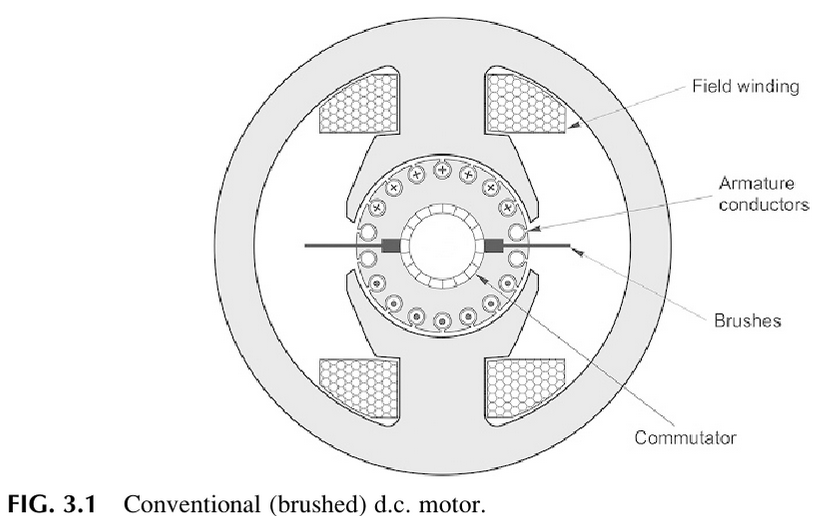
\includegraphics[width=0.4\linewidth]{../../figures/HD-fig3_1.png}
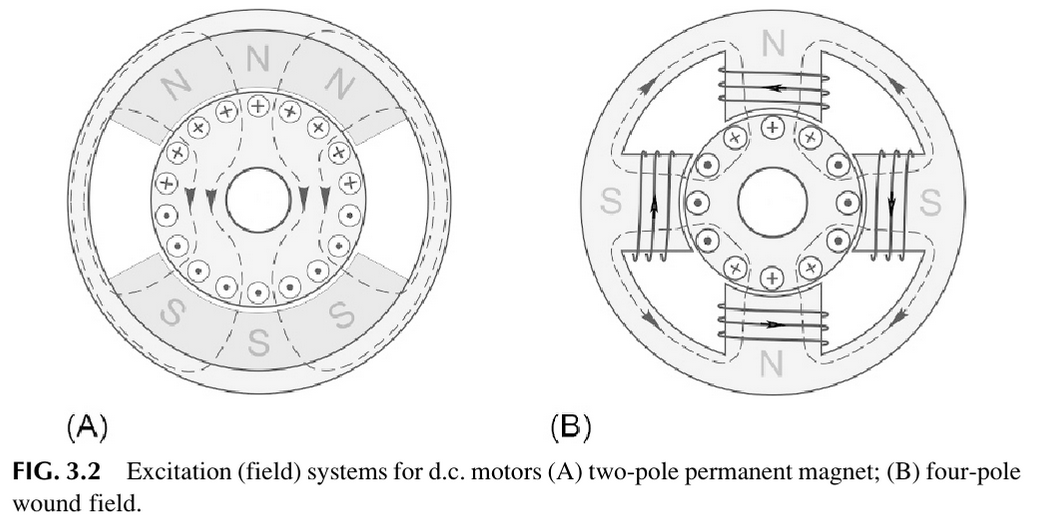
\includegraphics[width=0.53\linewidth]{../../figures/HD-fig3_2.png}
\end{center}
\end{frame}

\begin{frame}[label={sec:org08baf61}]{Circuito equivalente}
\begin{center}
  \begin{circuitikz}
    \draw (4,1) node[elmech](motor){M};
    \draw (motor.north) to[R=$R$] (4,4) to[L=$L$] (0,4)
    to[american voltage source, label=$V$] (0,0) -| (motor.south);
    \draw[thick,->>](motor.right)--++(1,0)node[midway,above]{$\omega$};

    \node[] at (2, -0.8 cm) {\(L \frac{d}{dt}i(t) +  Ri(t) + k\omega(t) = V\)};

    \begin{scope}[xshift=8cm]
    \draw (4,1) node[elmech](motor){M};
    \draw (motor.north) to[R=$R$] (4,4) to[short] (0,4)
    to[american voltage source, label=$V$] (0,0) -| (motor.south);
    \draw[thick,->>](motor.right)--++(1,0)node[midway,above]{$\omega$};
    \node[] at (2, -0.8 cm) {\(Ri(t) + k\omega(t) = V\)};
    \end{scope}
  \end{circuitikz}
\end{center}


Newton: \(J\frac{d}{dt}\omega(t) &= ki(t) - T_l(t)\)
\end{frame}

\begin{frame}[label={sec:org725f7f6}]{Velocidad con carga constanta}
En steady-state: \(i(t) = I\), \(\omega(t) = \omega\).

\begin{align*}
RI + k\omega &= V\\
0 &= kI - T_l
\end{align*}

\alert{Actividad individual} Escribe la velocidad angular como función de la carga \(T_l\) y el voltaje \(V\).
\end{frame}

\begin{frame}[label={sec:org9741574}]{Velocidad con carga constanta}
\[ RI + k\omega = V, \qquad\qquad  0 = kI - T_l\]
Un motor especifico tiene el constante \(k=\unit{4}{\newton\meter\per\ampere}\) y resistencia \(R=\SI{1}{\ohm}\). Se aplica un voltaje de \(V=\unit{100}{\volt}\) sobre su armadura.


\alert{Actividad} Dibuje como la velocidad en estado estable depende de la carga \(T_l\). ¿Cuál es el par de parada?

\begin{center}
  \begin{tikzpicture}[xscale=0.8]
    \draw[->] (0, 0) -- (9, 0) node[right] {$T_l$ [\unit{}{\newton\meter}]};
    \draw[->] (0, 0) -- (0, 3) node[left] {$\omega$};
    \foreach \t in { 1, 2, ..., 8} {
    \draw (\t, 0) -- (\t, -0.1) node[below] {\t{}00};
    }
    \end{tikzpicture}

\end{center}
\end{frame}

\begin{frame}[label={sec:orga8c0099}]{Arranque}
Para un motor parada, la fuerza contraelectromotriz es cero, y solo la resistencia de la armadura limite la corriente.

    \begin{scope}[]
    \draw (4,1) node[elmech](motor){M};
    \draw (motor.north) to[R=$R$] (4,4) to[short] (0,4)
    to[american voltage source, label=$V$] (0,0) -| (motor.south);
    \draw[thick,->>](motor.right)--++(1,0)node[midway,above]{$\omega$};
    \node[] at (2, -0.8 cm) {\(Ri(t) + k\omega(t) = V\)};
    \end{scope}
  \end{circuitikz}
\end{center}


Hay que tener cuidado en el arranque para que la corriente no sube a niveles excedentes.
\end{frame}
\end{document}